\documentclass{scrartcl}
	%enthaelt eqnref{}-Operator
	\usepackage{amsmath}

	%ngerman fur Umlaute, Anf"hrungszeichen, etc.%
	\usepackage[ngerman]{babel}

	%siunitx fur SI-Einheitesnsystem%
	\usepackage{siunitx}
	\sisetup{
	    locale=DE,
	    separate-uncertainty=true,
    	per-mode=fraction
	}

	%wrapfig fuer schoene umflossene Figuren
	\usepackage{wrapfig}

	%graphicx fur Bildeinbindung%
	\usepackage{graphicx}

	%UTF-8 encoding
	%\usepackage[applemac]{inputenc}
	\usepackage[T1]{fontenc}
	\usepackage[utf8]{inputenc}
	\usepackage{lmodern}

	%enthaelt pfeile mit text
	\usepackage{amssymb}

	%ermoeglicht Hyperlinks - Schein aber KACKE zu sein :D
	\usepackage{url}

	%damit lualatex formeln richtig darstellt klappt anscheinend auch nicht :P
	%\usepackage{unicode-math}

	% Vertikal Tabellenzellen verbinden
	\usepackage{multirow}

	%Texteinzug vor Absatz entfernen%
	\parindent 0pt

\begin{document}
	
	\vspace*{3cm}

	\begin{center}
		\large
		TU Dortmund
	\end{center}

	\begin{center}
		\Huge
		V301 - Leerlaufspannung und Innenwiderstand von Spannungsquellen
	\end{center}

	\begin{center}
		\large
		Korrektur
	\end{center}

	\vspace{5cm} % Bei Korrektur nur 5cm foer schoeneres Layout sonst 6cm
	\begin{center}
		\begin{minipage}[b]{8cm}
			\Large
			Markus Stabrin \\
			\normalsize
			markus.stabrin@tu-dortmund.de \\

			\Large
			Kevin Heinicke\\
			\normalsize
			kevin.heinicke@tu-dortmund.de \\
			\\
			\\

			Versuchsdatum: 7. Mai 2013 \\
			\\
			Abgabedatum: 14. Mai 2013
		\end{minipage}
	\end{center}

	\thispagestyle{empty}

	\newpage

	\section{Einleitung} % (fold)
\label{sec:einleitung}
	In diesem Versuch werden Funktionsweise und Kenngr"o"sen des Geiger-M"uller-Z"ahlrohrs untersucht.
	Das Ger"at erm"oglicht die Messung der Intensit"at ionisierender Strahlung.
	Auf Grund des einfachen Aufbaus ist das Geiger-M"uller-Z"ahlrohr kosteng"unstig und wegen seiner Verbreitung besonders interessant.

\section{Theorie} % (fold)
\label{sec:theorie}
	Zun"achst soll die Funktionsweise grob beschrieben werden.

	\subsection{Aufbau}
	\label{subsec:aufbau}
		Das Instrument besteht aus einem Anodendraht, der von einem Kathodenzylinder umschlossen ist.
		Der Raum zwischen Draht und Zylinder ist mit einem Gasgemisch niedrigen Drucks gef"ullt, das sich leicht ionisieren l"asst.
		Es wird eine Spannung $U$ zwischen $\SI{300}{\volt}$ und $\SI{2000}{\volt}$ an Anode und Kathode angelegt, wodurch ein radialsymmetrisches Feld im Innern des Zylinders entsteht.
		Der Zylinder ist von einem Stahlmantel umgeben, wobei eine Stirnseite aus einer d"unnen Membran aus Mylar besteht.
		Hierdurch wird m"oglichst wenig Strahlung beim Eintritt absorbiert und Gleichzeitig der Niederdruck im Inneren des Z"ahlrohrs bewahrt.

		\begin{figure}[h]
			\centering
			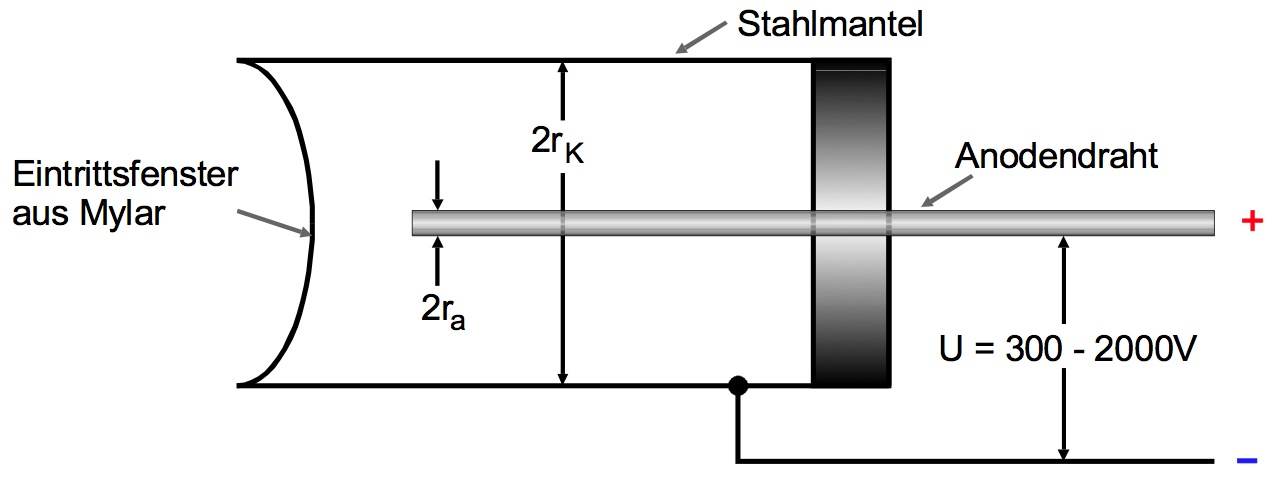
\includegraphics[width = 15cm]{img/zaehlrohr.jpeg}
			\caption{Querschnitt des Geiger-M"uller-Z"ahlrohrs \cite{anleitung}}
			\label{fig:querschnitt}
		\end{figure}

	\subsection{Funktionsweise}
	\label{subsec:funktionsweise}
		Wenn ein geladenes Teilchen in das Z"ahlrohr eintritt, gibt es seine Energie an die Gas\-atome ab und kann diese ionisieren, bis seine Energie aufgebraucht ist.
		Weil die Energie des einfallenden Teilchens wesentlich gr"o"ser ist, als die zur Ionisation ben"otigte Energie, ist die Anzahl ionisierter Kerne proportional zur Energie des Teilchens.
		Die freigesetzten Gas-Ionen werden nun durch das elektrische Feld abgelenkt und bei gen"ugend gro"ser Spannung $U$ in Anode und Kathode absorbiert.
		Die verschiedenen Wirkungsbereiche werden im Folgenden erl"autert.

		\begin{figure}[h]
			\centering
			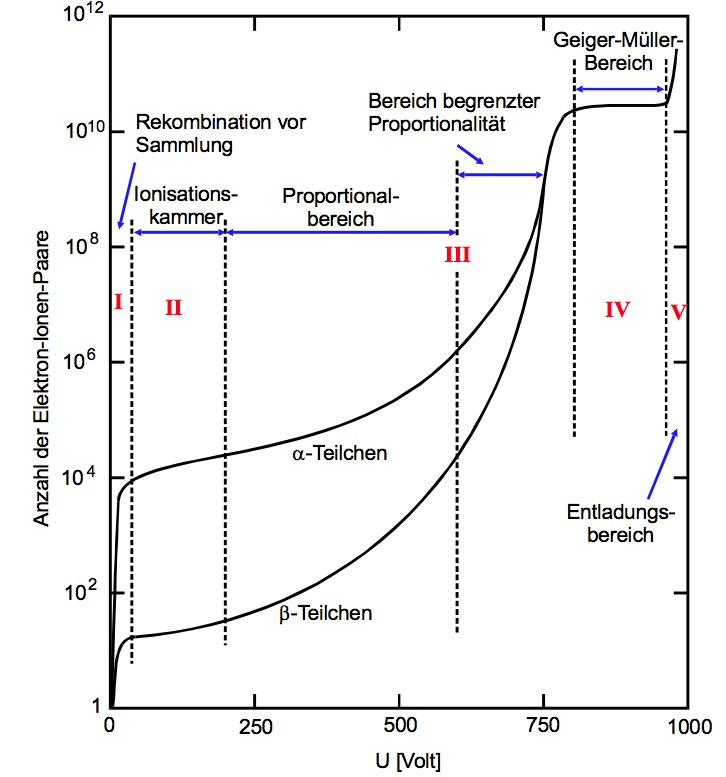
\includegraphics[width = 10cm]{img/bereiche.jpeg}
			\caption{Wirkungsbereiche des Geiger-M"uller-Z"ahlrohrs \cite{anleitung}}
			\label{fig:bereiche}
		\end{figure}

		\subsubsection{Rekombination (I)}
		\label{subsubsec:rekombination}
			Bei zu geringer angelegter Spannung (beim vorliegenden Ger"at $U < \SI{300}{\volt}$) reicht die Feldst"arke im Zylinder nicht aus, um die Ionen vollst"andig zu trennen.
			Sie rekombinieren und die einfallende Strahlung l"asst sich nicht detektieren.

		\subsubsection{Ionisationskammer (II)}
		\label{subsubsec:ionisationskammer}
			Erh"oht man die Spannung, wird jedes ionisierte Molek"ul absorbiert und der Strom zwischen Anode und Kathode ist proportional zur Energie und zur Intensit"at der einfallenden Strahlung.
			Da der auftretende Strom jedoch sehr gering ist, kann nur Strahlung hoher Intensit"at gemessen werden.
			Man bezeichnet das Z"ahlrohr dann als Ionisationskammer.

		\subsubsection{Proportionalit"atsbereich (III)}
		\label{subsubsec:proportionalitaetsbereich}
			Bei gr"o"serer Spannung haben die im Zylinder freigesetzten Elektronen gen"ugend Energie, um ihrerseits Molek"ule zu ionisieren.
			Auf diese Weise werden immer mehr Elektronen frei und man spricht man von einer \textsc{Townsend-Lawine}.
			Die Anzahl der freigesetzten Elektronen ist dabei nahezu proportional zur Energie der einfallenden Teilchen und die Spannung ist messbar gro"s.
			In diesem Bereich arbeitet der Detektor als Proportionalit"atsz"ahlrohr.

		\subsubsection{Geiger-M"uller-Bereich (IV)}
		\label{subsubsec:geiger-mueller-bereich}
			Wird die Spannung weiter erh"oht, entsteht bei den ersten Ionisationen eine Vielzahl von UV-Photonen, die sich im gesamten Z"ahlrohr ausbreiten und neue Elektronenlawinen ausl"osen.
			Die Ladung, die sich auf der Anode ansammelt, ist dann unabh"angig von der Energie des einfallenden Teilchens.
			Dieser Spannungsbereich wird auch als Ausl"osebereich bezeichnet und ist die haupts"achliche Verwendungsart des Geiger-M"uller-Z"ahlrohrs.
			Die Anzahl der gemessenen Teilchen ist hier nahezu konstant.
			Das so entstehende Plateau beschreibt die Charakteristik des Z"ahlrohrs.
			Ein langes Plateau mit geringer Steigung bedeutet dabei ein hochwertiges Z"ahlrohr.

			Bei noch h"oheren Spannungen wird durch ein einzelnes einfallendes Teilchen eine Dauerentladung gez"undet, wobei der anfallende Strom schlie"slich so stark wird, dass das Ger"at zerst"ort werden kann.

	\subsection{Nebeneffekte: Totzeit und Nachentladungen}
	\label{subsec:nebeneffekte}
		Ein unerw"unschter Effekt des Geiger-M"uller-Z"ahlrohrs wird als Totzeit bezeichnet.
		Weil die positiv geladenen Atomr"umpfe langsamer von der Kathode absorbiert werden, als die leichten Elektronen, bilden die R"umpfe f"ur eine kurze Zeit eine Ladungswolke, die dem elektrischen Feld entgegenwirkt.
		Dies macht weitere Ionisationen unm"oglich.

		Zudem werden bei der Absorption der Atomr"umpfe in der Zylinderh"ulle m"oglicherweise Elektronen herausgeschlagen.
		Diese durchlaufen das gesamte Potential und k"onnen wiederum eine Lawine und damit einen messbaren Spannungsimpuls hervorrufen, der das Ergebnis verf"alscht.
		Diesem als Nachentladung bezeichneten Effekt wird durch die Zugabe eines Alkohol-Gases entgegengewirkt.

	\subsection{Ansprechverm"ogen}
	\label{subsec:ansprechvermoegen}
		Das Ansprechverm"ogen bezeichnet die Wahrscheinlichkeit, mit der ein Teilchen detektiert werden kann.
		Weil $\alpha-$ und $\beta-$Strahlung aus vergleichsweise gro"sen Teilchen besteht, wird diese zu nahezu $\SI{100}{\percent}$ nachgewiesen.
		Das Ansprechverm"ogen f"ur Photonen liegt dagegen nur bei etwa $\SI{1}{\percent}$, weshalb hier nur sehr hohe Intensit"aten gemessern werden k"onnen.

		Durch die in \ref{subsec:aufbau} erw"ahnte, d"unne Membran an der Eintrittsseite des Zylinders wird gew"ahrleistet, dass m"oglichst viele Teilchen die Z"ahlkammer erreichen.

	\section{Versuchsaufbau und Durchf"uhrung} % (fold)
\label{sec:durchfuehrung}

\subsection{Direkte Messung der Leerlaufspannung} % (fold)
\label{sub:direkte_messung_der_leerlaufspannung}

\begin{wrapfigure}{r}{7cm}
	\centering
	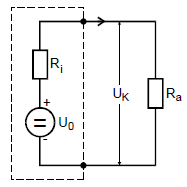
\includegraphics[width = 5cm]{img/Monozelle.PNG}
	\caption{Schaltbild zur direkten Messung der Leerlaufspannung. \cite{anleitung}}
	\label{aufgabea}
\end{wrapfigure}{r}

Die Schaltung wird nach Abb.\ref{aufgabea} aufgebaut. Der Widerstand $R_\mathrm{a}$ entspricht hierbei dem Eingangswiderstand $R_\mathrm{v}$ des hochohmigen Spannungsmessger"ates.
Es werden $U_\mathrm{k}$ und $R_\mathrm{v}$ notiert.

\newpage

\subsection{Messung der Leerlaufspannung und des Innenwiderstandes mittels eines variablen Widerstandes} % (fold)
\label{sub:messung_der_leerlaufspannung_mittels_eines_variablen_widerstandes_}

\begin{wrapfigure}{r}{7cm}
	\centering
	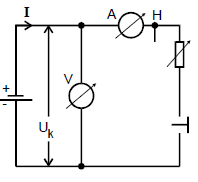
\includegraphics[width = 5cm]{img/b.PNG}
	\caption{Messchaltung zur Bestimmung von $U_\mathrm{0}$ und $R_\mathrm{i}$ \cite{anleitung}.}
	\label{aufgabeb}
\end{wrapfigure}

Die Schaltung wir nach Abb.\ref{aufgabeb} aufgebaut.
Der variable Belastungswiderstand liegt dabei in einem Bereich von $\SI{0}{\ohm}$ bis $\SI{50}{\ohm}$. Es werden bei 10 verschiedenen Belastungswiderst"anden $R_\mathrm{k}$ die Klemmenspannung $U_\mathrm{k}$ in Abh"angigkeit von dem Belastungsstrom $I$ aufgenommen.

\subsection{Messung der Leerlaufspannung und des Innenwiderstandes mittels eines variablen Widerstandes und einer Gegenspannung} % (fold)
\label{sub:messung_der_leerlaufspannung_mittels_eines_variablen_widerstandes_}

\begin{wrapfigure}{r}{7cm}
	\centering
	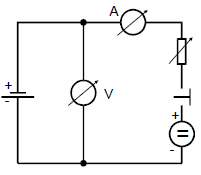
\includegraphics[width = 5cm]{img/c.PNG}
	\caption{Messchaltung zur Bestimmung von $U_\mathrm{0}$ und $R_\mathrm{i}$ mittels einer Gegenspannung \cite{anleitung}.}
	\label{aufgabec}
\end{wrapfigure}

Die Schaltung wird nach Abb.\ref{aufgabec} aufgebaut.
Die Gegenspannung soll dabei etwa $\SI{2}{\volt}$ gr"o"ser sein als die Leerlaufspannung $U_\mathrm{0}$.
Es werden bei 10 verschiedenen Belastungswiderst"anden $R_\mathrm{k}$ die Klemmenspannung $U_\mathrm{k}$ in Abh"angigkeit von dem Belastungsstrom $I$ aufgenommen.

\subsection{Sinus- und Rechteckausgang} % (fold)
\label{sub:sinus_und_rechteckausgang}

Die Schaltung wird nach Abb.\ref{aufgabeb} aufgebaut.
Nun wird jedoch ein Sinus- bzw. Rechtecksspannungsgenerator angeschlossen.

F"ur die Messung mit der Rechtecksspannung wird ein variabler Widerstand von $\SI{20}{\ohm}$ bis $\SI{250}{\ohm}$ benutzt.

Bei der Messung mit der Sinusspannung hingegen einer mit einem Bereich von $\SI{0.1}{\kilo\ohm}$ bis $\SI{5}{\kilo\ohm}$.

Es werden bei 10 verschiedenen Belastungswiderst"anden $R_\mathrm{k}$ die Klemmenspannung $U_\mathrm{k}$ in Abh"angigkeit von dem Belastungsstrom $I$ aufgenommen.

	\section{Auswertung}
\label{sec:auswertung}


\begin{table}[!h]
\begin{center}
\begin{tabular}{|r|r|r|r|}
\hline
Puls-Echo & & Durchschall & \\
\hline
\hline
 L"ange[$\SI{}{\milli\meter}$] & Laufzeit[$\SI{}{\micro\second}$] & L"ange[$\SI{}{\milli\meter}$] & Laufzeit[$\SI{}{\micro\second}$]\\
\hline
\hline
 39,65 &	15,60 &	 39,65 &	16,6\\
 80,40 &	30,55 &	 80,40 &	31,7\\
120,40 &	45,15 &	120,40 &	46,4\\
\hline
\end{tabular}
\caption[]{Me"sergebnisse zur Bestimmung der Schallgeschwindigkeit in Acrylglas der 1Mhz Sonde.}
\label{a1}
\end{center}
\end{table}

\begin{table}[!h]
\begin{center}
\begin{tabular}{|r|r|}
\hline
 L"ange[$\SI{}{\milli\meter}$] & Laufzeit[$\SI{}{\micro\second}$]\\
\hline
\hline
39.65 &	15.15\\
39.65 &	15.40\\
80.40 &	30.10\\
80.40 &	30.80\\
120.4 &	44.75\\
120.4 &	45.50\\
\hline
\end{tabular}
\caption[]{Me"sergebnisse zur Bestimmung der Schallgeschwindigkeit in Acrylglas der 2Mhz Sonde.}
\label{a2}
\end{center}
\end{table}

\begin{table}[!h]
\begin{center}
\begin{tabular}{|r|r|r|r|}
\hline
Puls-Echo & & Durchschall &\\
\hline
 L"ange[$\SI{}{\milli\meter}$] & Laufzeit[$\SI{}{\micro\second}$] & L"ange[$\SI{}{\milli\meter}$] & Laufzeit[$\SI{}{\micro\second}$]\\
\hline
\hline
 39,65 &	14,85 &	 39,65 &	15,4\\
 80,40 &	29,75 &	 80,40 &	30,3\\
120,40 &	44,35 &	120,40 &	44,9\\
\hline
\end{tabular}
\caption[]{Me"sergebnisse zur Bestimmung der Schallgeschwindigkeit in Acrylglas der 4Mhz Sonde.}
\label{a4}
\end{center}
\end{table}

\begin{table}[!h]
\begin{center}
\begin{tabular}{|r|r|r|r|r|r|}
\hline
 $\SI{1}{\mega\hertz}$ && $\SI{2}{\mega\hertz}$ && $\SI{3}{\mega\hertz}$&\\
\hline
Peak1[$\SI{}{\micro\second}$] & Peak2[$\SI{}{\micro\second}$] & Peak1[$\SI{}{\micro\second}$] & Peak2[$\SI{}{\micro\second}$] & Peak1[$\SI{}{\micro\second}$] & Peak2[$\SI{}{\micro\second}$]\\
\hline
\hline
42.1 &	13.2 &	40.9 &	12.2 &	40.6 &	11.8\\
12.2 &	48.2 &	11.2 &	47.1 &	10.9 &	46.6\\
18.2 &	42.3 &	17.1 &	41.2 &	16.7 &	40.7\\
24.1 &	36.4 &	23.0 &	35.3 &	22.6 &	34.8\\
30.1 &	30.5 &	29.0 &	29.3 &	28.5 &	28.9\\
35.5 &	24.4 &	34.4 &	23.2 &	33.9 &	22.8\\
41.2 &	18.0 &	40.0 &	16.8 &	39.5 &	16.4\\
46.5 &	11.7 &	45.5 &	10.7 &	45.0 &	10.4\\
15.0 &	46.3 &	14.0 &	45.6 &	13.6 &	45.1\\
16.1 &	45.5 &	15.3 &	44.4 &	14.9 &	43.8\\
\hline
\end{tabular}
\caption[]{Durch das Puls-Echo Verfahren erhaltene Werte zur Bestimmung der Lochgr"o"se.}
\label{loch1}
\end{center}
\end{table}
\begin{table}[!h]
\begin{center}
\begin{tabular}{|r|r|r|r|r|r|}
\hline
$\frac{1}{2}t_\mathrm{1}[\SI{}{\micro\second}$] & $\frac{1}{2}t_\mathrm{2}[\SI{}{\micro\second}$] & $s_\mathrm{eff,1}[\SI{}{\milli\meter}]$ & $\Delta s_\mathrm{eff,1}[\SI{}{\milli\meter}]$ & $s_\mathrm{eff,2}[\SI{}{\milli\meter}]$ & $\Delta s_\mathrm{eff,2}[\SI{}{\milli\meter}]$ \\ 
\hline
\hline
21.05 &	 6.60 &	57.28 &	0.08 &	17.95 &	0.02 \\
 6.10 &	24.10 &	16.59 &	0.02 &	65.57 &	0.09 \\
 9.10 &	21.15 &	24.76 &	0.03 &	57.55 &	0.08 \\
12.05 &	18.20 &	32.78 &	0.04 &	49.52 &	0.06 \\
15.05 &	15.25 &	40.95 &	0.05 &	41.49 &	0.05 \\
17.75 &	12.20 &	48.30 &	0.06 &	33.19 &	0.04 \\
20.60 &	 9.00 &	56.05 &	0.07 &	24.49 &	0.03 \\
23.25 &	 5.85 &	63.26 &	0.08 &	15.91 &	0.02 \\
 7.50 &	23.15 &	20.40 &	0.02 &	62.99 &	0.08 \\
 8.05 &	22.75 &	21.90 &	0.03 &	61.90 &	0.08 \\
 \hline
 \hline
$s_\mathrm{1}[\SI{}{\milli\meter}]$ & $\Delta s_\mathrm{1}[\SI{}{\milli\meter}]$ & $s_\mathrm{2}[\SI{}{\milli\meter}]$ & $\Delta s_\mathrm{2}[\SI{}{\milli\meter}]$ & b[$\SI{}{\milli\meter}$] & $\Delta$b[$\SI{}{\milli\meter}$]\\
\hline
\hline
55.18 &	0.10 &	15.85 &	0.06 &	8.66 &	0.24\\
14.49 &	0.06 &	63.48 &	0.11 &	1.72 &	0.24\\
22.66 &	0.07 &	55.45 &	0.10 &	1.58 &	0.24\\
30.69 &	0.07 &	47.42 &	0.09 &	1.58 &	0.23\\
38.85 &	0.08 &	39.39 &	0.08 &	1.45 &	0.23\\
46.20 &	0.09 &	31.09 &	0.07 &	2.40 &	0.23\\
53.95 &	0.10 &	22.39 &	0.07 &	3.35 &	0.24\\
61.16 &	0.10 &	13.81 &	0.06 &	4.71 &	0.24\\
18.30 &	0.06 &	60.89 &	0.10 &	0.50 &	0.24\\
19.80 &	0.07 &	59.80 &	0.10 &	0.09 &	0.24\\
\hline
\end{tabular}
\caption[]{Daten zur Bestimmung der Lochbreiten b mit einer $\SI{1}{\mega\hertz}$ Sonde. Dabei ist $s_\mathrm{eff}$ die Strecke inklusive des Sondenwegs, $s$ die Strecke ohne Sondenweg, $t$ die Laufzeit und $b$ die Lochbreite.}
\label{loch1}
\end{center}
\end{table}
\begin{table}[!h]
\begin{center}
\begin{tabular}{|r|r|r|r|r|r|}
\hline
$\frac{1}{2}t_\mathrm{1}[\SI{}{\micro\second}$] & $\frac{1}{2}t_\mathrm{2}[\SI{}{\micro\second}$] & $s_\mathrm{eff,1}[\SI{}{\milli\meter}]$ & $\Delta s_\mathrm{eff,1}[\SI{}{\milli\meter}]$ & $s_\mathrm{eff,2}[\SI{}{\milli\meter}]$ & $\Delta s_\mathrm{eff,2}[\SI{}{\milli\meter}]$ \\ 
\hline
\hline
21.05 &	 6.60 &	55.32 &	0.23 &	16.50 &	0.07 \\
 6.10 &	24.10 &	15.15 &	0.07 &	63.71 &	0.26 \\
 9.10 &	21.15 &	23.13 &	0.10 &	55.73 &	0.23 \\
12.05 &	18.20 &	31.11 &	0.13 &	47.75 &	0.20 \\
15.05 &	15.25 &	39.23 &	0.16 &	39.63 &	0.17 \\
17.75 &	12.20 &	46.53 &	0.19 &	31.38 &	0.13 \\
20.60 &	 9.00 &	54.10 &	0.22 &	22.72 &	0.10 \\
23.25 &	 5.85 &	61.54 &	0.25 &	14.47 &	0.06 \\
 7.50 &	23.15 &	18.94 &	0.08 &	61.68 &	0.25 \\
 8.05 &	22.75 &	20.70 &	0.09 &	60.06 &	0.25 \\
 \hline
 \hline
$s_\mathrm{1}[\SI{}{\milli\meter}]$ & $\Delta s_\mathrm{1}[\SI{}{\milli\meter}]$ & $s_\mathrm{2}[\SI{}{\milli\meter}]$ & $\Delta s_\mathrm{2}[\SI{}{\milli\meter}]$ & b[$\SI{}{\milli\meter}$] & $\Delta$b[$\SI{}{\milli\meter}$]\\
\hline
\hline
54.44 &	0.42 &	15.62 &	0.36 &	9.64 &	0.59\\
14.27 &	0.36 &	62.82 &	0.44 &	2.61 &	0.61\\
22.25 &	0.37 &	54.84 &	0.42 &	2.61 &	0.60\\
30.23 &	0.38 &	46.86 &	0.41 &	2.61 &	0.59\\
38.34 &	0.39 &	38.75 &	0.39 &	2.61 &	0.59\\
45.65 &	0.41 &	30.50 &	0.38 &	3.56 &	0.59\\
53.22 &	0.42 &	21.84 &	0.37 &	4.64 &	0.60\\
60.66 &	0.44 &	13.59 &	0.36 &	5.45 &	0.60\\
18.05 &	0.37 &	60.80 &	0.44 &	0.85 &	0.60\\
19.81 &	0.37 &	59.17 &	0.43 &	0.72 &	0.60\\
\hline
\end{tabular}
\caption[]{Daten zur Bestimmung der Lochbreite b mit einer $\SI{2}{\mega\hertz}$ Sonde. Dabei ist $s_\mathrm{eff}$ die Strecke inklusive des Sondenwegs, $s$ die Strecke ohne Sondenweg, $t$ die Laufzeit und $b$ die Lochbreite.}
\label{loch1}
\end{center}
\end{table}
\begin{table}[!h]
\begin{center}
\begin{tabular}{|r|r|r|r|r|r|}
\hline
$\frac{1}{2}t_\mathrm{1}[\SI{}{\micro\second}$] & $\frac{1}{2}t_\mathrm{2}[\SI{}{\micro\second}$] & $s_\mathrm{eff,1}[\SI{}{\milli\meter}]$ & $\Delta s_\mathrm{eff,1}[\SI{}{\milli\meter}]$ & $s_\mathrm{eff,2}[\SI{}{\milli\meter}]$ & $\Delta s_\mathrm{eff,2}[\SI{}{\milli\meter}]$ \\ 
\hline
\hline
21.05 &	 6.60 &	55.57 &	0.03 &	16.15 &	0.01 \\
 6.10 &	24.10 &	14.92 &	0.01 &	63.78 &	0.03 \\
 9.10 &	21.15 &	22.86 &	0.01 &	55.70 &	0.03 \\
12.05 &	18.20 &	30.93 &	0.02 &	47.63 &	0.02 \\
15.05 &	15.25 &	39.01 &	0.02 &	39.55 &	0.02 \\
17.75 &	12.20 &	46.40 &	0.02 &	31.20 &	0.02 \\
20.60 &	 9.00 &	54.06 &	0.03 &	22.45 &	0.01 \\
23.25 &	 5.85 &	61.59 &	0.03 &	14.23 &	0.01 \\
 7.50 &	23.15 &	18.61 &	0.01 &	61.73 &	0.03 \\
 8.05 &	22.75 &	20.39 &	0.01 &	59.95 &	0.03 \\
 \hline
 \hline
$s_\mathrm{1}[\SI{}{\milli\meter}]$ & $\Delta s_\mathrm{1}[\SI{}{\milli\meter}]$ & $s_\mathrm{2}[\SI{}{\milli\meter}]$ & $\Delta s_\mathrm{2}[\SI{}{\milli\meter}]$ & b[$\SI{}{\milli\meter}$] & $\Delta$b[$\SI{}{\milli\meter}$]\\
\hline
\hline
54.69 &	0.04 &	15.27 &	0.03 &	9.75 &	0.21\\
14.04 &	0.03 &	62.90 &	0.05 &	2.77 &	0.21\\
21.97 &	0.03 &	54.82 &	0.04 &	2.90 &	0.21\\
30.05 &	0.04 &	46.75 &	0.04 &	2.90 &	0.21\\
38.12 &	0.04 &	38.67 &	0.04 &	2.90 &	0.21\\
45.52 &	0.04 &	30.32 &	0.04 &	3.86 &	0.21\\
53.18 &	0.04 &	21.56 &	0.03 &	4.96 &	0.21\\
60.71 &	0.04 &	13.35 &	0.03 &	5.64 &	0.21\\
17.73 &	0.03 &	60.84 &	0.04 &	1.12 &	0.21\\
19.51 &	0.03 &	59.06 &	0.04 &	1.12 &	0.21\\
\hline
\end{tabular}
\caption[]{Daten zur Bestimmung der Lochbreiten b mit einer $\SI{4}{\mega\hertz}$ Sonde. Dabei ist $s_\mathrm{eff}$ die Strecke inklusive des Sondenwegs, $s$ die Strecke ohne Sondenweg, $t$ die Laufzeit und $b$ die Lochbreite.}
\label{loch4}
\end{center}
\end{table}
\begin{table}[!h]
\begin{center}
\begin{tabular}{|r|r|r|r|}
\hline
Puls-Echo & & Durchschall & \\
\hline
\hline
$v_\mathrm{e}$[$\SI{}{\milli\meter\per\micro\per\second}$] & $\delta$s[$\SI{}{\milli\meter}$] & $v_\mathrm{d}$[$\SI{}{\milli\meter\per\micro\per\second}$]& $\delta$s[$\SI{}{\milli\meter}$]\\
\hline
$\SI{2.733 (4)}{}$ & $\SI{3.013 (132)}{}$ & $\SI{2.710 (6)}{}$ & $\SI{5.386 (219)}{}$\\
\hline
\hline
&&&\\
$\bar{\mathrm{v}}$ & $\SI{2.721 (4)}{}$ & $\bar{\delta s}$ & $\SI{4.199 (128)}{}$\\
\hline
$\delta$t & $\SI{1.543 (47)}{}$ & &\\
\hline
\end{tabular}
\caption[]{Ergebnisse der linearen Regression f"ur die $\SI{1}{\mega\hertz}$ Sonde.}
\label{r1}
\end{center}
\end{table}
\begin{table}[!h]
\begin{center}
\begin{tabular}{|r|r|r|r|}
\hline
Puls-Echo & & Durchschall & \\
\hline
\hline
$v_\mathrm{e}$[$\SI{}{\milli\meter\per\micro\per\second}$] & $\delta$s[$\SI{}{\milli\meter}$] & $v_\mathrm{d}$[$\SI{}{\milli\meter\per\micro\per\second}$]& $\delta$s[$\SI{}{\milli\meter}$]\\
\hline
$\SI{2.728 (1)}{}$ & $\SI{1.691 (43)}{}$ & $\SI{2.682 (22)}{}$ & $\SI{1.84306 (713)}{}$\\
\hline
\hline
&&&\\
$\bar{\mathrm{v}}$[$\SI{}{\milli\meter\per\micro\per\second}$] & $\SI{2.705 (11)}{}$ & $\bar{\delta s}$[$\SI{}{\milli\meter}$] & $\SI{1.767 (357)}{}$\\
\hline
$\delta$t & $\SI{0.653 (132)}{}$ &&\\
\hline
\end{tabular}
\caption[]{Ergebnisse der linearen Regression f"ur die $\SI{2}{\mega\hertz}$ Sonde.}
\label{r2}
\end{center}
\end{table}
\begin{table}[!h]
\begin{center}
\begin{tabular}{|r|r|r|r|}
\hline
Puls-Echo & & Durchschall & \\
\hline
\hline
v[$\SI{}{\milli\meter\per\micro\per\second}$] & $\delta$s[$\SI{}{\milli\meter}$] & v[$\SI{}{\milli\meter\per\micro\per\second}$]& $\delta$s[$\SI{}{\milli\meter}$]\\
\hline
$\SI{2.737 (1)}{}$ & $\SI{1.010 (44)}{}$ & $\SI{2.737 (1)}{}$ & $\SI{2.516 (45)}{}$\\
\hline
\hline
\\
$\bar{\mathrm{v}}$[$\SI{}{\milli\meter\per\micro\per\second}$] & $\SI{2.737 (1)}{}$ & $\bar{\delta s}$[$\SI{}{\milli\meter}$] & $\SI{1.763 (32)}{}$\\
\hline
\end{tabular}
\caption[]{Ergebnisse der linearen Regression f"ur die $\SI{4}{\mega\hertz}$ Sonde.}
\label{r4}
\end{center}
\end{table}
\begin{table}[!h]
\begin{center}
\begin{tabular}{|r|r|r|r|r|}
\hline
Sonde[$\SI{}{\mega\hertz}$] & Peak1[$\SI{}{\micro\second}$] & Peak2[$\SI{}{\micro\second}$] & Peak3[$\SI{}{\micro\second}$] & Peak4[$\SI{}{\micro\second}$]\\
\hline
\hline
1 &	12.4 &	18.3 &	26.3 &	72.8\\
2 &	12.0 &	17.6 &	24.4 &	71.7\\
4 &	11.7 &	16.6 &	24.8 &	71.1\\
\hline
\end{tabular}
\caption[]{Messdaten zur Berechnung der Ma"se der Nachbildung eines Auges.}
\label{auge1}
\end{center}
\end{table}

\begin{table}[!h]
\begin{center}
\begin{tabular}{|r|r|r|r|r|r|}
\hline
Sonde[$\SI{}{\mega\hertz}$] & $d_\mathrm{S,I}[\SI{}{\milli\meter}]$ & $d_\mathrm{I,L1}[\SI{}{\milli\meter}]$ & $d_\mathrm{L1,L2}[\SI{}{\milli\meter}]$ & $d_\mathrm{L2,R}[\SI{}{\milli\meter}]$ & $d_\mathrm{ges}[\SI{}{\milli\meter}]$\\
\hline
\hline
1 &	7.66 &	4.16 &	10.00 & 32.78 &	54.60\\
2 & 8.00 &	3.95 &	 8.50 &	33.35 &	53.80\\
4 &	7.79 &	3.45 &	10.25 & 32.64 &	54.13\\
\hline
\end{tabular}
\caption[]{Abmessungen des Auges mithilfe verschiedener Ultraschallsonden. Dabei ist $d_\mathrm{S,I}$ der Abstand zwischen Sonde und Iris, $d_\mathrm{I,L1}$ der Abstand zwischen Iris und Linse1, $d_\mathrm{L1,L2}$ der Abstand zwischen Anfang der Linse und Ende der Linse, $d_\mathrm{L2,R}$ der Abstand zwischen Ende der Linse und der Retina.}
\label{auge2}
\end{center}
\end{table}

	\newpage
\section{Diskussion}
	\label{sec:diskussion}
	Dieser Versuch stellt eine M"oglichkeit zur Bestimmung der Viskosit"at von Wasser vor.
	Alle damit ermittelten Werte liegen weit "uber den Literaturwerten \cite{uni_magdeburg}.
	Bei $T = \SI{20}{\celsius}$ lag die Abweichung bei $\SI{19}{\percent}$.
	Mit steigender Temperatur vergr"o"serte sich der Unterschied sogar noch und stieg bei $T = \SI{54}{\celsius}$ auf etwa $\SI{22}{\percent}$ an.
	Diese Unterschiede lassen sich nur duch systematische Fehler erkl"aren.
	Die Messung liefert also insgesamt eher schlechte Werte.	

\begin{thebibliography}{9}
	\bibitem{anleitung} Physikalisches Anf"angerpraktikum der TU Dortmund: Versuch Nr. 107 - Das Kugelfallviskosimeter nach H"oppler. Stand: November 2012.

	\bibitem{uni_magdeburg} Universit"at Magdeburg, Institut f"ur Str"omungsmechanik und Thermodynamik: Stoffwerte von Wasser. www.uni-magdeburg.de/isut/LSS/Lehre/Arbeitsheft/IV.pdf. Stand: 2. Dezember 2012.

	\bibitem{walcher} Walcher, W.: Praktikum der Physik. Teubner Studienb"ucher, Teubner-Verlag. Stuttgart.
\end{thebibliography}

\end{document}